\documentclass[11pt]{article}
% chktex-file 29 chktex-file 36
% (29: kernel/algorithm names like Philox-4x32 and ampere_sgemm_128x64
%  legitimately use 'x'; 36: parens in \texttt{...()} are code references.)

% Allow line breaks inside \url and \path at hyphens and other punctuation.
% Must be set before hyperref (which loads the url package internally).
\PassOptionsToPackage{hyphens}{url}

\usepackage[margin=1in]{geometry}
\usepackage{amsmath,amssymb,mathtools}
\usepackage{graphicx}
\usepackage{booktabs}
\usepackage{array}
\usepackage{tabularx}
\usepackage{float}
\usepackage{xcolor}
\usepackage{hyperref}
\usepackage{microtype}
\usepackage{enumitem}
\usepackage{listings}
\usepackage[T1]{fontenc}
\usepackage{lmodern}

% Let URL spacing stretch a bit to avoid overfull boxes from long identifiers.
\Urlmuskip=0mu plus 1mu\relax

\hypersetup{
	colorlinks=true,
	linkcolor=blue!55!black,
	citecolor=blue!55!black,
	urlcolor=blue!55!black
}

\lstdefinestyle{pythonstyle}{
	language=Python,
	basicstyle=\ttfamily\small,
	breaklines=true,
	frame=single,
	columns=fullflexible,
	keepspaces=true,
	showstringspaces=false,
	backgroundcolor=\color{gray!6},
	rulecolor=\color{gray!35}
}

\setlist[itemize]{leftmargin=*}
\setlist[enumerate]{leftmargin=*}
\newcolumntype{L}[1]{>{\raggedright\arraybackslash}p{#1}}
\newcolumntype{Y}{>{\raggedright\arraybackslash}X}

\title{GPU-Accelerated Martingale Posterior Neural Processes for MNIST Image Completion}
\author{Jose Perales\\EN605.617: Introduction to GPU Programming\\Johns Hopkins University}
\date{Spring 2026}

\begin{document}

\maketitle

\begin{abstract}
	The Martingale Posterior Neural Process (MPNP, Lee et al., ICLR 2023)
	replaces the arbitrary latent prior of a standard Neural Process with
	predictive resampling. At every training step the model draws synthetic
	context sets from its own predictive distribution and refits. The payoff
	is calibrated, prior-free uncertainty over functions. An MPNP provides
	calibrated doubt, not just inference, the kind a deployed model needs
	before it brakes for a pedestrian, flags a tumor, or sizes a tail-risk
	position. The cost is that every gradient step now runs many encoder and
	decoder forward passes per task, making the model GPU-bound.

	This paper takes a working PyTorch MPNP implementation for MNIST image
	completion and uses it as a vehicle for a tour of the CUDA stack. It
	walks through which NVIDIA library kernel each MPNP op actually
	launches: cuBLAS \texttt{cublasGemmEx} GEMMs for the MLPs, native ATen
	softmax and LayerNorm kernels for the attention blocks, TensorIterator
	elementwise kernels for the loss, the in-tree Philox RNG, and the
	caching allocator. Pseudo-context resampling multiplies those launches
	by $K{+}2$ every training step, which is what makes MPNP GPU-bound in
	the first place.
\end{abstract}

\section{Introduction}

Models that return only a point estimate are often unsuitable in risky
environments. Autonomous driving needs a confidence band on the
pedestrian-detection score before it commits to braking. In clinical
decision support, a model that flags its own uncertainty is more useful
than one that is confidently wrong. Quantitative finance needs tail risk
that is calibrated, not just estimated. Uncertainty quantification is
critical wherever predictions inform consequential actions.

Lee, Yun, Nam, Fong, and Lee provide a solution to uncertainty
quantification with the Martingale Posterior Neural Process (MPNP)
~\cite{lee2023}, a Bayesian-style Neural Process that does not require a
prior. Following Fong, Holmes, and Walker~\cite{fong2023}, they replace
the prior with predictive resampling. At every step, the model generates
$K$ synthetic context sets from its own predictive distribution, refits,
and uses the spread of refits as the posterior. Posterior updates form a
martingale (expected belief over self-generated data does not drift). The
result is coherent uncertainty without ever specifying a prior.

However, predictive resampling comes at a computational cost. The new
objective requires pseudo-context forward passes through the encoder,
decoder, and per-target Gaussian negative log-likelihood (NLL) per task
per training step. This is a natural fit for the GPU, and it makes MPNP
a useful case study in GPU programming. This paper traces how a PyTorch
implementation maps onto the CUDA stack underneath: which library each
MPNP op dispatches to, and which call sites the pseudo-context loop
multiplies.

\section{Math Review}

\subsection{Martingale Posterior Distributions}

Classical Bayesian inference asks ``what do I believe about the
parameter $\theta$?''; a question that demands a prior $\pi(\theta)$
before any data is observed. Fong, Holmes, and Walker flip the question:
``how do I expect future observations to look, given what data I already
have?'' That requires only a one-step predictive
$P_n(\cdot \mid y_{1:n})$, no prior~\cite{fong2023}.

Uncertainty about $\theta$ becomes uncertainty about the missing future.
Fong et al.~design a predictive resampling mechanism to forward-simulate
a long imaginary future from the current predictive, refit, and read off
$\theta$:

\begin{equation}
	Y_i \sim P_{i-1}, \quad i = n{+}1, \dots, N
	\quad\Longrightarrow\quad
	\theta_N = \theta(P_N) \sim \Pi_N(\cdot \mid y_{1:n}).
\end{equation}

Repeating the simulation many times yields a full posterior $\Pi_N$ over
$\theta$. The predictive sequence $\{P_n\}$ is a
\href{https://en.wikipedia.org/wiki/Martingale_(probability_theory)}{martingale},
$\mathbb{E}\!\left[P_{n+1} \mid P_n\right] = P_n$, so beliefs are
consistent and do not drift on self-generated data. There is no prior to
choose and no likelihood to specify, only a predictive model and the
samples it generates.

\subsection{Neural Processes}

The two classical answers to this problem space (predictions with calibrated uncertainty)
each have a flaw. Neural networks are flexible, scalable function
approximators but return only point predictions with no principled
uncertainty. Gaussian processes give exact posterior mean and variance
per query but cost $\mathcal{O}(n^3)$ per task and do not amortize across
datasets.

Neural Processes (NPs)~\cite{garnelo2018} sit in the middle. Like a
Gaussian Process, an NP learns a distribution over functions from a
context set $\mathcal{C} = {\{(x_i, y_i)\}}_{i=1}^{n}$, but it does so
with a neural network and amortizes inference into a single forward
pass:

\begin{equation}
	p(y_t \mid x_t, \mathcal{C}) = \int p(y_t \mid x_t, z)\,
	q(z \mid \mathcal{C})\, dz.
\end{equation}

A permutation-invariant encoder $q_\phi(z \mid \mathcal{C})$ (MLP plus
mean-pool) maps the context set to a latent distribution, and a decoder
$p_\theta(y_t \mid x_t, z)$ predicts each target from the latent. The
model is trained by maximizing an evidence lower bound. The remaining
problem is the same one Bayesian inference always has. The latent prior
$p(z)$ is arbitrary, so the posterior is rarely calibrated.

\subsection{Martingale Posterior Neural Processes}

Lee et al.\ plug Fong's predictive resampling inside the NP training loop
~\cite{lee2023}. The model uses the same encoder and decoder, plus a
pseudo-context generator, an Induced Set Attention Block (ISAB)
~\cite{lee2019set}, that samples $K$ synthetic context sets
$\mathcal{Z}_0^{(k)}$ from the model's own current predictive. This is a
neural analogue of predictive resampling.

The training objective combines three terms:

\begin{equation}
	\boxed{\mathcal{L}_{\text{MPNP}} =
	\underbrace{\mathcal{L}_{\text{amort}}}_{\text{predict from real }\mathcal{C}}
	+
	\underbrace{\mathcal{L}_{\text{marg}}}_{\substack{\text{log-mean-exp over }K\\\text{pseudo-augmentations}}}
	+
	0.1 \cdot
	\underbrace{\mathcal{L}_{\text{pseudo}}}_{\substack{\text{pseudo}\to\text{target}\\\text{consistency}}}.}
\end{equation}

Here
\begin{align}
	\mathcal{L}_{\text{amort}}
	 & = -\mathbb{E}_{q(z\mid\mathcal{C})}\left[\log p(y_T \mid x_T, z)\right], \\
	\mathcal{L}_{\text{marg}}
	 & = -\log\left(\frac{1}{K}\sum_{k=1}^{K} p(y_T \mid x_T, \theta_k)\right),
	\qquad \theta_k = \theta\left(\mathcal{C} \cup \mathcal{Z}_0^{(k)}\right),
\end{align}
and $\mathcal{L}_{\text{pseudo}}$ scores the predictive quality of the
pseudo-set alone.

$\mathcal{L}_{\text{marg}}$ requires $K$ pseudo-augmented forward passes
per task per step. With $B = 64$, $T = 784$, hidden width $h = 256$, and
$K = 5$, the inner forward graph holds
$\mathcal{O}(B \cdot K \cdot T \cdot h)$ activations and launches at
least $K{+}1$ separate sequences of linear-layer, decode, and log-prob
kernels per step. This is the bottleneck that the rest of the paper
targets.

\section{MNIST Example}

\subsection{Task Formulation}

Each $28\times28$ MNIST image is flattened into 784 coordinate-intensity
pairs:

\begin{itemize}
	\item $x_i \in {[-1, 1]}^2$: normalized pixel coordinate (row, column).
	\item $y_i \in [0, 1]$: pixel intensity.
\end{itemize}

Per training task, a random subset of $n \in [10, 300]$ pixels is
revealed as context. The model must predict all 784 pixel intensities
and their per-pixel standard deviations. MNIST is a fitting test bed for
a Neural Process because it has variable-size context, genuine spatial
structure, and uncertainty that should localize on unobserved pixels and
ambiguous edges.

\subsection{Architecture and Hyperparameters}

The \href{../martingale_posterior_neural_process.py}{MPNP implementation}
reuses the encoder/decoder MLPs from
\href{../neural_process.py}{\path{neural_process.py}}, adapted from Dupont's
NP repository~\cite{dupont}. The pseudo-context generator is a single ISAB
block built from two \texttt{MAB} (multihead-attention block) layers with 8
heads.

The shapes that appear throughout Section~\ref{sec:cuda} are listed in
Table~\ref{tab:tensor-shapes}.

\begin{table}[H]
	\centering
	\begin{tabular}{lll}
		\toprule
		Tensor           & Shape                    & Notes                  \\
		\midrule
		context $(x, y)$ & $(B, n, 3)$              & $n$ varies per batch   \\
		target $x_T$     & $(B, 784, 2)$            & fixed                  \\
		target $y_T$     & $(B, 784, 1)$            & fixed                  \\
		pseudo-context   & $(B, K, M, 3)$           & $K{=}5$, $M{=}30$      \\
		latent $z$       & $(B, K, z_{\text{dim}})$ & $z_{\text{dim}}{=}256$ \\
		\bottomrule
	\end{tabular}
	\caption{Tensor shapes used by the MPNP training step.}\label{tab:tensor-shapes}
\end{table}

Hyperparameters from \href{../train_inpainting.py}{\texttt{train\_inpainting.py}}
are listed in Table~\ref{tab:hyperparameters}.

\begin{table}[H]
	\centering
	\begin{tabular}{ll}
		\toprule
		Hyperparameter           & Value                                                                                                    \\
		\midrule
		Hidden width $h = r = z$ & 256                                                                                                      \\
		Pseudo-points $M$        & 30                                                                                                       \\
		Pseudo-samples $K$       & 5                                                                                                        \\
		Loss weights             & $(\mathcal{L}_{\text{amort}}, \mathcal{L}_{\text{marg}}, \mathcal{L}_{\text{pseudo}}) = (1.0, 1.0, 0.1)$ \\
		Optimizer                & AdamW, lr $5{\times}10^{-4}$, weight decay $10^{-5}$                                                     \\
		LR schedule              & Cosine, $T_{\max} = 150$                                                                                 \\
		Batch size               & 64                                                                                                       \\
		Epochs                   & 150                                                                                                      \\
		Gradient clip            & $\|g\|_2 \le 5$                                                                                          \\
		Train / val / test split & 50 000 / 10 000 / 10 000                                                                                 \\
		\bottomrule
	\end{tabular}
	\caption{Training hyperparameters.}\label{tab:hyperparameters}
\end{table}

\subsection{Qualitative Results}

After 150 epochs the model reaches a test NLL of $-1.941$ (best
validation NLL $-1.947$ at epoch 145; approximately 100.66~s/epoch over
approximately 4.19~h on a single GPU). Lower is better, and for a
Gaussian over $[0, 1]$ pixels this corresponds to $\sigma$ in the low
tens of percent on average.

\begin{figure}[H]
	\centering
	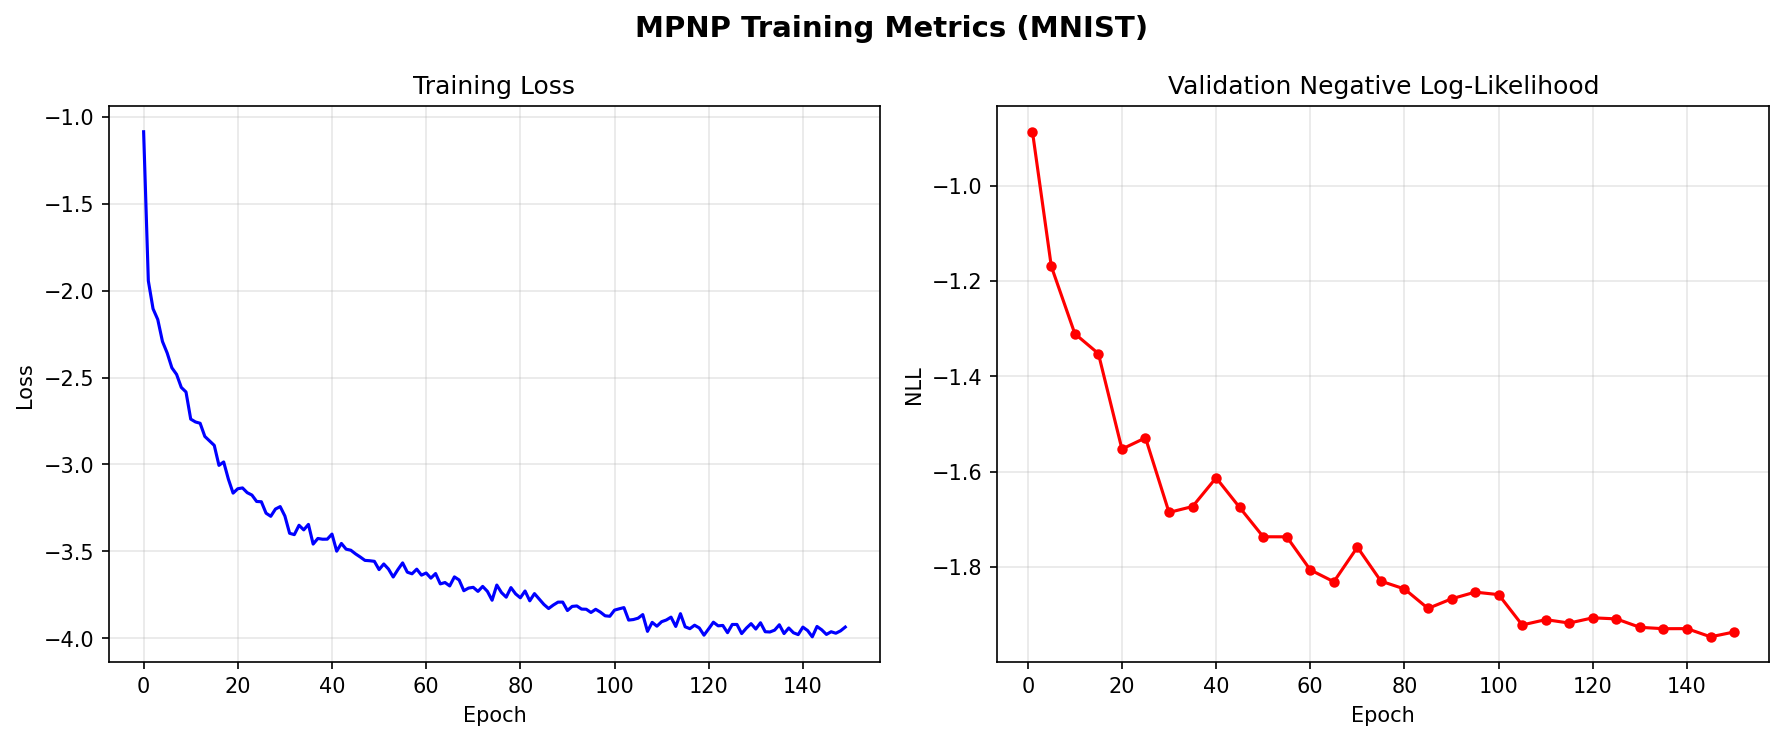
\includegraphics[width=0.92\linewidth]{../output/training_metrics.png}
	\caption{Training loss and validation NLL across 150 epochs. Loss
		decreases smoothly; validation NLL tracks training loss with no
		prior-collapse pathology and no overfitting.}\label{fig:training-metrics}
\end{figure}

\begin{figure}[H]
	\centering
	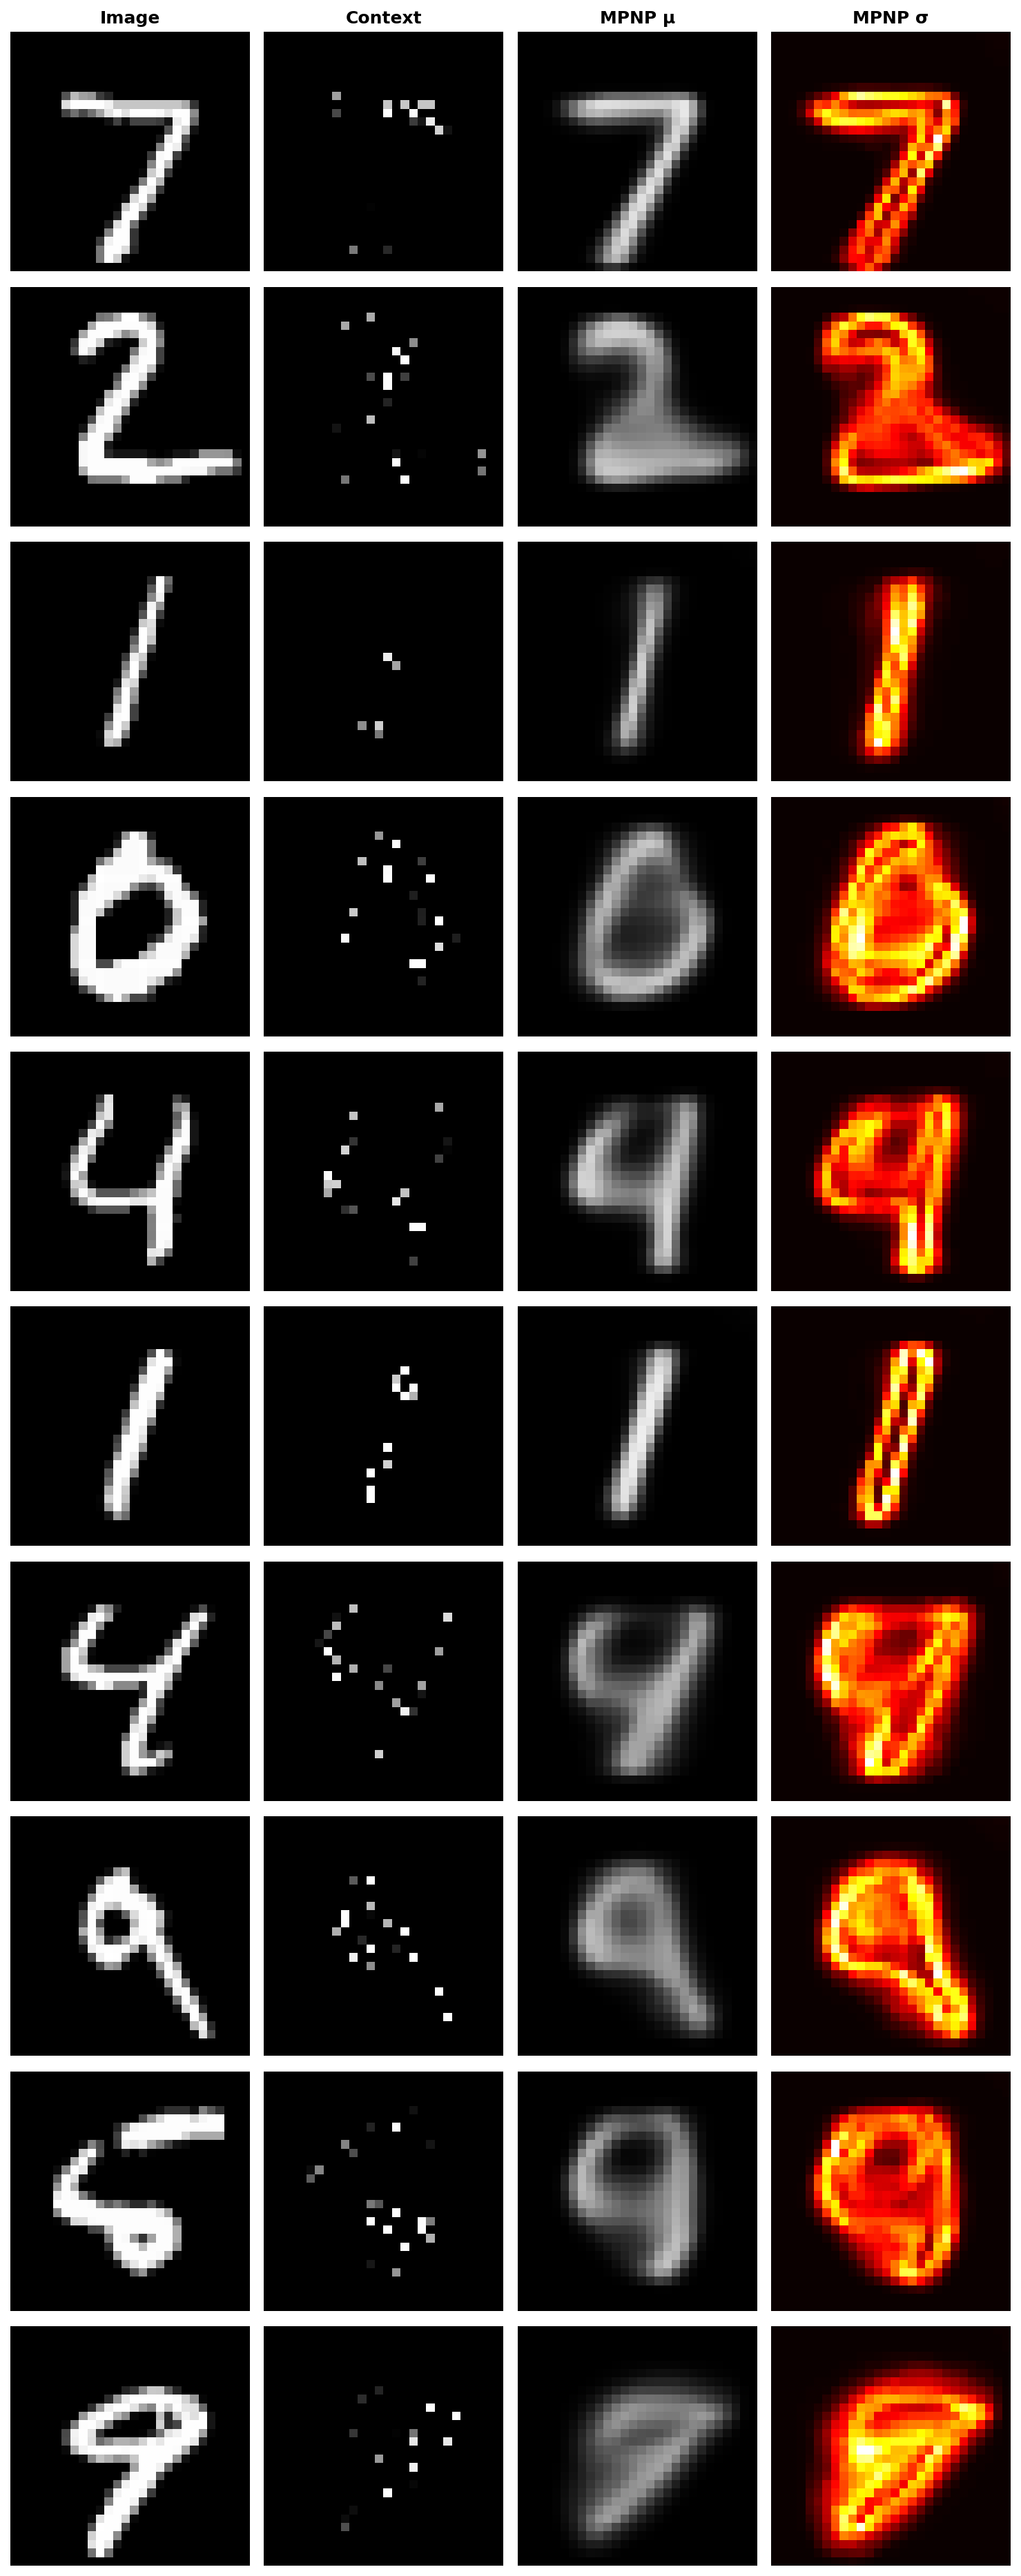
\includegraphics[width=0.45\linewidth]{../output/mpnp_mnist_completion.png}
	\caption{Test-set image completion. Columns: original digit, observed
		context pixels, predicted mean $\mu$, predicted standard deviation
		$\sigma$. Uncertainty concentrates on unobserved regions and on
		ambiguous strokes, matching the calibration behavior reported by the
		MPNP paper.}\label{fig:completion}
\end{figure}

The remainder of the paper analyzes how this training loop runs on the
GPU\@.

\section{CUDA Programming inside PyTorch}\label{sec:cuda}

\begin{sloppypar}
	The MPNP implementation in
	\href{../train_inpainting.py}{\path{train_inpainting.py}} and
	\href{../martingale_posterior_neural_process.py}{\path{martingale_posterior_neural_process.py}}
	abstracts over all the CUDA programming covered in this course, yet a
	single training step issues dozens of CUDA kernel launches across
	cuBLAS, the caching allocator, and ATen's library of elementwise and
	reduction kernels. This section inventories the GPU-touching call
	sites and names the backend behind each one.
\end{sloppypar}

\subsection{The PyTorch, ATen, CUDA dispatch stack}\label{subsec:stack}

Before naming individual kernels it helps to fix the layering, because
the project itself contains no CUDA C++ code. Every tensor operation
flows through three layers~\cite{ezyang,pytorchdispatcher}:

\begin{enumerate}
	\item \textbf{Python / \texttt{torch.nn}.} The user-facing API
	      (\texttt{nn.Linear}, \texttt{Normal.log\_prob},
	      \texttt{loss.backward()}). Each call constructs an op and hands it
	      to ATen.
	\item \textbf{ATen} (\emph{A Tensor library}). PyTorch's C++ op
	      library and dispatcher~\cite{atencppdocs,pytorchdispatcher}. For each
	      op (\texttt{aten::addmm}, \texttt{aten::mean}, \texttt{aten::log},
	      \ldots) ATen looks at the input tensors' device and dtype and
	      routes the call to a backend implementation. The \texttt{aten::}
	      prefix visible in profiler output is just this namespace.
	\item \textbf{CUDA backend.} The actual GPU code. For CUDA tensors,
	      ATen routes either to a vendor library shipped by NVIDIA
	      (cuBLAS for GEMM~\cite{cublas}, cuDNN for convolutions and some
	      normalizations~\cite{cudnn})
	      or to one of ATen's own native CUDA kernels for ops NVIDIA does
	      not provide, such as the \texttt{TensorIterator} elementwise and
	      reduction kernels~\cite{ezyang} behind \texttt{add}, \texttt{mul},
	      \texttt{log}, \texttt{mean}, and so on, dedicated kernels for
	      \texttt{softmax} and \texttt{layer\_norm}, and the in-tree
	      Philox-4x32 random-number generator~\cite{cudasem}.
\end{enumerate}

The practical consequence is that every kernel inventoried in the rest
of this section comes from one of those two sources --- a vendor
library or an ATen native CUDA kernel --- and reasoning about cost
means knowing which.

\subsection{Where the GPU runs in this project}\label{subsec:where}

Almost every line of
\texttt{train\_inpainting.py} and
\texttt{martingale\_posterior\_neural\_process.py} exercises
the GPU, in three distinct phases: the data path, the forward path,
and the loss-and-backward path.

\paragraph{Data path.} The MNIST point cloud is built on the CPU\@.
\texttt{MNISTPointCloud.\_\_init\_\_} pre-computes a $784 \times 2$
coordinate grid as a CPU tensor; \texttt{\_\_getitem\_\_} returns a
CPU \texttt{(coords, values)} pair. The DataLoader is constructed
with \texttt{pin\_memory=True}, which routes those CPU batches through
page-locked host memory so the subsequent \verb|x_full.to(device)| in
\texttt{train\_epoch} can issue an asynchronous \texttt{cudaMemcpyAsync}
instead of a blocking copy~\cite{cudasem}. The synthetic
\texttt{torch.randperm(n, device=x.device)} call inside
\texttt{context\_target\_split} runs the permutation on the GPU using
the in-tree Philox-4x32 generator that backs PyTorch's CUDA RNG~\cite{curand}.

\paragraph{Forward path.} A single training step calls
\path{model.compute_loss(x_ctx, y_ctx, x_tgt, y_tgt)}, which in
turn invokes \texttt{encode\_set} once on the real context, then
$K{=}5$ more times on each combined context, plus \texttt{decoder}
calls in matching number. Each of those calls is a stack of
\texttt{nn.Linear} layers separated by \texttt{ReLU} activations; each
\texttt{nn.Linear} dispatches to \texttt{aten::addmm}, which is a
cuBLAS GEMM with bias fusion~\cite{cublas}. The mean-pool aggregator inside
\texttt{encode\_set} is a single \texttt{aten::mean} reduction. The
hand-written \texttt{MultiHeadAttention} block inside the
\texttt{ISAB} pseudo-context generator issues two
\texttt{aten::matmul} kernels, an \texttt{aten::softmax}, and several
small reshapes. The reparameterization
$z = \mu + \sigma \odot \epsilon$ inside \texttt{q\_context.rsample()}
is one elementwise kernel scheduled through \texttt{TensorIterator}~\cite{ezyang}.

\paragraph{Loss and backward path.} \texttt{Normal.log\_prob(y\_tgt)}
expands into a sequence of elementwise kernels (\texttt{log},
\texttt{pow}, \texttt{sub}, \texttt{div}) followed by an
\texttt{aten::mean} reduction; this fires $K{+}1$ times per step. The
marginal-likelihood term in \texttt{compute\_loss} stacks $K$ such
log-likelihoods and reduces them with a hand-rolled log-sum-exp
(\texttt{max} $\to$ \texttt{sub} $\to$ \texttt{exp} $\to$
\texttt{mean} $\to$ \texttt{log}, four kernels where
\texttt{torch.logsumexp} would be one). Calling
\texttt{loss.backward()} traverses the autograd graph in reverse and
launches the gradient kernel for each forward op above on the same
CUDA stream the forward used~\cite{cudasem}. The
\texttt{optimizer.step()} call on \texttt{torch.optim.AdamW} fires a
fused multi-tensor elementwise kernel that updates every parameter in
one launch.

Table~\ref{tab:kernel-map} summarizes the mapping. The shapes use the
project's actual hyperparameters: batch size $B{=}64$, hidden width
$h{=}256$, context size $n \in [10, 300]$, target size $T{=}784$
pixels per image, latent width $z{=}256$, $M{=}30$ pseudo-context
points, $8$ attention heads, and $K{=}5$ pseudo-context samples.

\begin{table}[H]
	\centering
	\small
	\setlength{\tabcolsep}{3pt}
	\begin{tabularx}{\linewidth}{@{}L{0.18\linewidth}L{0.14\linewidth}YL{0.18\linewidth}@{}}
		\toprule
		MPNP step & ATen op                                                         & Backend / kernel & Tensor shape \\
		\midrule
		Encoder MLP (\texttt{Linear} + \texttt{ReLU})
		          & \texttt{addmm}
		          & cuBLAS \texttt{cublasGemmEx}~\cite{cublas}
		          & $(B{\cdot}n,256)$ ${\times}(256,256)$                                                             \\
		\addlinespace
		Mean-pool over context
		          & \texttt{mean}
		          & ATen reduction, \texttt{\_\_shfl\_down\_sync}~\cite{coopgroups}
		          & $(B,n,256)$ ${\to}(B,256)$                                                                        \\
		\addlinespace
		ISAB MAB stack (${\times}K$)
		          & \texttt{matmul}, \texttt{softmax}, \texttt{layer\_norm}
		          & cuBLAS batched GEMM + ATen CUDA kernels~\cite{cublas}
		          & $(B,8,30,32)$                                                                                     \\
		\addlinespace
		Reparam.\ $z{=}\mu{+}\sigma\epsilon$
		          & \texttt{add}, \texttt{mul}
		          & TensorIterator + Philox-4x32~\cite{ezyang}
		          & $(B,256)$                                                                                         \\
		\addlinespace
		Decoder MLP
		          & \texttt{addmm}
		          & cuBLAS \texttt{cublasGemmEx}~\cite{cublas}
		          & $(B{\cdot}T,256)$ ${\times}(256,256)$                                                             \\
		\addlinespace
		Per-pixel Gaussian NLL
		          & \texttt{log}, \texttt{pow}, \texttt{sub}
		          & TensorIterator elementwise~\cite{ezyang}
		          & $(B,784,1)$                                                                                       \\
		\addlinespace
		Manual log-sum-exp over $K$
		          & \texttt{max}, \texttt{exp}, \texttt{log}
		          & 5 ATen kernels in sequence
		          & $(K,B)$                                                                                           \\
		\addlinespace
		AdamW step
		          & \texttt{\_foreach\_*}
		          & multi-tensor elementwise
		          & all params                                                                                        \\
		\bottomrule
	\end{tabularx}
	\caption{Mapping from MPNP operations to PyTorch ops, CUDA backend kernels, and tensor shapes.}\label{tab:kernel-map}
\end{table}

Two structural facts about this table matter. First, the encoder,
decoder, and per-pixel log-likelihood each fire $K{+}2$ times per
training step (once for the real context pass and $K$ more times
inside the pseudo-context loop) so any per-launch cost is multiplied
accordingly. Second, the only ops whose tensor shapes vary
batch-to-batch are the encoder GEMM and the mean-pool reduction (both
because $n$ varies); every other shape is fixed by the architecture.

\section{Conclusion}

After 150 epochs the model reaches a test NLL of $-1.941$ with stable
training, and image completions (Figure~\ref{fig:completion})
reproduce the qualitative behavior of the original MPNP paper:
predicted $\sigma$ concentrates on unobserved regions and ambiguous
edges, the calibrated-uncertainty pattern that motivates the method.

The exercise also makes the implicit CUDA stack underneath PyTorch
concrete. Every \texttt{nn.Linear} in the encoder and decoder is a
cuBLAS GEMM, every \texttt{Normal.log\_prob} is a chain of
TensorIterator elementwise kernels, and every \texttt{torch.randperm}
draw runs through the in-tree Philox generator. Pseudo-context
resampling multiplies all of those launches by $K{+}2$ per step,
which is what makes MPNP a useful vehicle for the tour rather than
just another MNIST model.

\begin{thebibliography}{99}
	\raggedright{}

	\bibitem{lee2023}
	H. Lee, E. Yun, G. Nam, E. Fong, and J. Lee.
	\newblock{}Martingale Posterior Neural Processes.
	\newblock{}\emph{International Conference on Learning Representations}, 2023.
	\newblock{}\url{https://arxiv.org/abs/2304.09431}.

	\bibitem{fong2023}
	E. Fong, C. Holmes, and S. G. Walker.
	\newblock{}Martingale Posterior Distributions.
	\newblock{}\emph{Journal of the Royal Statistical Society: Series B}, 2023.
	\newblock{}\url{https://arxiv.org/abs/2103.15671}.

	\bibitem{garnelo2018}
	M. Garnelo, J. Schwarz, D. Rosenbaum, F. Viola, D. J. Rezende, S. M. A. Eslami,
	and Y. W. Teh.
	\newblock{}Neural Processes.
	\newblock{}\emph{ICML Workshop}, 2018.
	\newblock{}\url{https://arxiv.org/abs/1807.01622}.

	\bibitem{lee2019set}
	J. Lee, Y. Lee, J. Kim, A. Kosiorek, S. Choi, and Y. W. Teh.
	\newblock{}Set Transformer: A Framework for Attention-based Permutation-Invariant Neural Networks.
	\newblock{}\emph{International Conference on Machine Learning}, 2019.
	\newblock{}\url{https://arxiv.org/abs/1810.00825}.

	\bibitem{dupont}
	E. Dupont.
	\newblock{}Neural Processes (PyTorch).
	\newblock{}\url{https://github.com/EmilienDupont/neural-processes}.

	\bibitem{cudasem}
	PyTorch documentation.
	\newblock{}CUDA semantics notes.
	\newblock{}\url{https://docs.pytorch.org/docs/stable/notes/cuda.html}.

	\bibitem{ezyang}
	E. Z. Yang.
	\newblock{}PyTorch internals.
	\newblock{}2019.
	\newblock{}\url{https://blog.ezyang.com/2019/05/pytorch-internals/}.

	\bibitem{cublas}
	NVIDIA Corporation.
	\newblock{}cuBLAS Library User Guide.
	\newblock{}\url{https://docs.nvidia.com/cuda/cublas/}.

	\bibitem{coopgroups}
	K. Patel and S. Jones.
	\newblock{}Cooperative Groups: Flexible CUDA Thread Programming.
	\newblock{}NVIDIA Developer Blog, 2017.
	\newblock{}\url{https://developer.nvidia.com/blog/cooperative-groups/}.

	\bibitem{curand}
	NVIDIA Corporation.
	\newblock{}cuRAND Library User Guide.
	\newblock{}\url{https://docs.nvidia.com/cuda/curand/}.

	\bibitem{cudnn}
	NVIDIA Corporation.
	\newblock{}cuDNN Developer Guide.
	\newblock{}\url{https://docs.nvidia.com/deeplearning/cudnn/}.

	\bibitem{atencppdocs}
	PyTorch documentation.
	\newblock{}PyTorch C++ API (ATen).
	\newblock{}\url{https://pytorch.org/cppdocs/}.

	\bibitem{pytorchdispatcher}
	PyTorch documentation.
	\newblock{}Registering a Dispatched Operator in C++.
	\newblock{}\url{https://pytorch.org/tutorials/advanced/dispatcher.html}.

\end{thebibliography}

\end{document}
